\documentclass{article}
\usepackage{tikz}
\usetikzlibrary{babel,positioning,shapes.multipart,calc,arrows.meta,external}

\tikzexternalize[shell escape=-enable-write18] % activate externalisation

\tikzset{external/system call={pdflatex \tikzexternalcheckshellescape -halt-on-error
-interaction=batchmode -jobname "\image" "\texsource" && 
pdftops -eps "\image.pdf"}}

\begin{document}
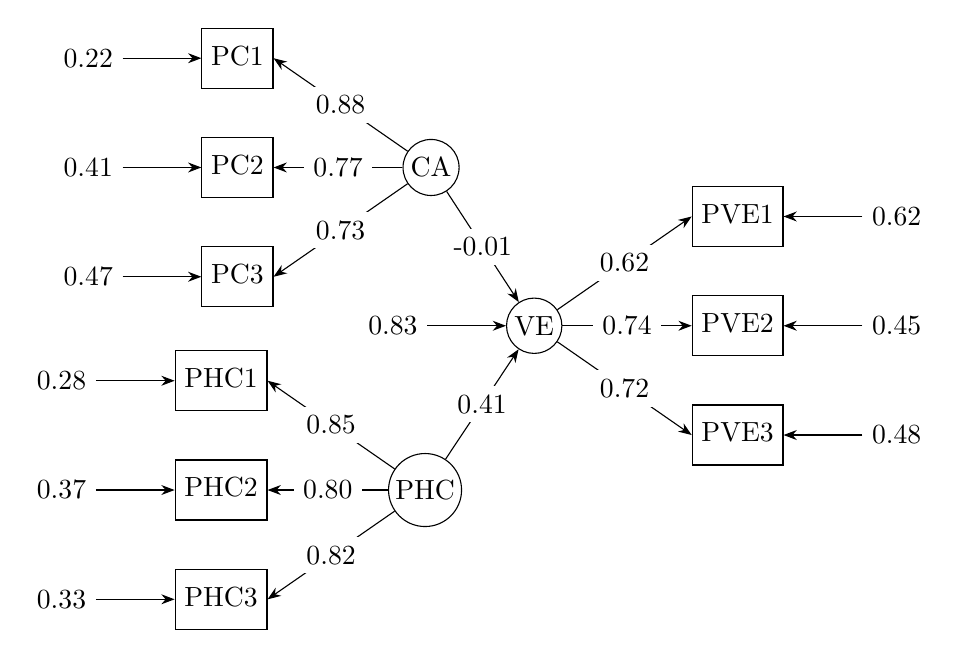
\begin{tikzpicture}
    [
    basic/.style={draw, text centered},
    circ/.style={basic, circle, minimum size=2em, inner sep=1.5pt},
    rect/.style={basic, text height=1em, text depth=.5em, minimum width=1.5em},
    >={Stealth[]}
    ]

    % Variables latentes
    \node [circ] (ve) {VE};
    \node [circ, above left=1.5cm and 0.8cm of ve] (ca) {CA};
    \node [circ, below left=1.5cm and 0.8cm of ve] (phc) {PHC};
    \draw [->] (ca) -- node[fill=white] {-0.01} (ve);
    \draw [->] (phc) -- node[fill=white] {0.41} (ve);
    % Variancia de VE
    \node [left=of ve] (delta) {0.83};
    \draw [->] (delta) -- (ve);
    % Variables indicadoras de VE
    \node [rect, above right=1cm and 2cm of ve.center] (pve1) {PVE1};
    \node [rect, right=2cm of ve.center] (pve2) {PVE2};
    \node [rect, below right=1cm and 2cm of ve.center] (pve3) {PVE3};
    \draw [->] (ve) -- node[fill=white] {0.62} (pve1.west);
    \draw [->] (ve) -- node[fill=white] {0.74} (pve2.west);
    \draw [->] (ve) -- node[fill=white] {0.72} (pve3.west);
    % Variancia de variables indicadoras de VE
    \node [right=of pve1] (epve1) {0.62};
    \node [right=of pve2] (epve2) {0.45};
    \node [right=of pve3] (epve3) {0.48};
    \draw [->] (epve1) -- (pve1);
    \draw [->] (epve2) -- (pve2);
    \draw [->] (epve3) -- (pve3);
    % Variables indicadoras de CA
    \node [rect, above left=1cm and 2cm of ca.center] (pc1) {PC1};
    \node [rect, left=2cm of ca.center] (pc2) {PC2};
    \node [rect, below left=1cm and 2cm of ca.center] (pc3) {PC3};
    \draw [->] (ca) -- node[fill=white] {0.88} (pc1.east);
    \draw [->] (ca) -- node[fill=white] {0.77} (pc2.east);
    \draw [->] (ca) -- node[fill=white] {0.73} (pc3.east);
    % Variancia de variables indicadoras de CA
    \node [left=of pc1] (epc1) {0.22};
    \node [left=of pc2] (epc2) {0.41};
    \node [left=of pc3] (epc3) {0.47};
    \draw [->] (epc1) -- (pc1);
    \draw [->] (epc2) -- (pc2);
    \draw [->] (epc3) -- (pc3);
    % Variables indicadoras de PHC
    \node [rect, above left=1cm and 2cm of phc.center] (phc1) {PHC1};
    \node [rect, left=2cm of phc.center] (phc2) {PHC2};
    \node [rect, below left=1cm and 2cm of phc.center] (phc3) {PHC3};
    \draw [->] (phc) -- node[fill=white] {0.85} (phc1.east);
    \draw [->] (phc) -- node[fill=white] {0.80} (phc2.east);
    \draw [->] (phc) -- node[fill=white] {0.82} (phc3.east);
    % Variancia de variables indicadoras de CA
    \node [left=of phc1] (ephc1) {0.28};
    \node [left=of phc2] (ephc2) {0.37};
    \node [left=of phc3] (ephc3) {0.33};
    \draw [->] (ephc1) -- (phc1);
    \draw [->] (ephc2) -- (phc2);
    \draw [->] (ephc3) -- (phc3);
\end{tikzpicture}
\end{document}